% ****** Start of file apssamp.tex ******
%
%   This file is part of the APS files in the REVTeX 4 distribution.
%   Version 4.0 of REVTeX, August 2001
%
%   Copyright (c) 2001 The American Physical Society.
%
%   See the REVTeX 4 README file for restrictions and more information.
%
% TeX'ing this file requires that you have AMS-LaTeX 2.0 installed
% as well as the rest of the prerequisites for REVTeX 4.0
%
% See the REVTeX 4 README file
% It also requires running BibTeX. The commands are as follows:
%
%  1)  latex apssamp.tex
%  2)  bibtex apssamp
%  3)  latex apssamp.tex
%  4)  latex apssamp.tex
%
\documentclass[twocolumn,showpacs,preprintnumbers,amsmath,amssymb,pre]{revtex4-1}
%\documentclass[preprint,showpacs,preprintnumbers,amsmath,amssymb, 12pt, linenumbers]{revtex4-1}

% Some other (several out of many) possibilities
%\documentclass[preprint,aps] {revtex4}
%\documentclass[preprint,aps,draft]{revtex4}
%\documentclass[prb]{revtex4}% Physical Review B
\usepackage{graphicx}% Include figure files
\usepackage{epstopdf}
\usepackage{dcolumn}% Align table columns on decimal point
\usepackage{bm}% bold math
\usepackage{color}
\usepackage{forloop}
\usepackage{amsfonts}

\definecolor{blue}{RGB}{0, 0, 150}
\definecolor{green}{RGB}{0,150,0}
\definecolor{red}{RGB}{200, 0, 0}
\definecolor{black}{RGB}{0, 0, 0}
%\nofiles

%%%%%%%%%%%% Yen Ting's Latex module %%%%%%%%%%%%%%%
\newcommand{\pr}[1]{\mathbb{P}\left\{#1\right\}}
\newcommand{\E}[1]{\mathbb{E}\left[#1\right]}
\newcommand{\var}[1]{\text{var} \left[ #1 \right]}
\renewcommand{\l}{\left}
\renewcommand{\r}{\right}
\newcommand{\subeq}[2]{\begin{subequations}\label{#2}\begin{align}#1\end{align}\end{subequations}}
\newcommand{\eq}[2]{\begin{equation}#1\label{#2}\end{equation}}
\newcommand{\al}[2]{\begin{align}#1\label{#2}\end{align}}
\newcommand{\blue}[1]{{\color{blue}{#1}}}
\newcommand{\red}[1]{{\color{red}{#1}}}
\newcommand{\green}[1]{{\color{green}{#1}}}
\newcommand{\black}[1]{{\color{black}{#1}}}
\newcommand{\smal} [1]{{\small #1}}
\newcommand{\YT}[1]{{\blue{#1}}}
%%%%%%%%%%%%%%%%  END %%%%%%%%%%%%%%%%%%%%%

\begin{document}

\section{Fermi--Dirac Statistics of Rod Orientations} \label{sec:FD}
\newcommand{\vx}{{\bf r}}
\newcommand{\ve}{{\bf e}}
We use a bead-and-rod model to model the chromosomes. Each chromosome consists of $N$ beads freely jointed by $N$ rods forming a loop; the rod length is chosen to be the Kuhn length $\Delta l$ of of the DNA. 
The position of the $i^{\rm th}$ bead is denote by $\vx_i$, and without lost of generality, the spindle pole body is defined to be the $0^{\rm th}$ bead. The topology of the polymer forming a look suggests a periodic condition $\vx_0=\vx_N$. We do not consider volume exclusion in this model. We shall define the the direction of the $i^{\rm th}$ rod to be $\ve_i:=\vx_{i+1} - \vx_{i}$.  In a one-dimensional setting, $\vx_i = x_i \Delta l$ where $x_i \in \mathbb{Z}$, and $\ve_i=\pm \Delta l$ for $i=0, 1, \ldots, N-1$. 

The spindle pole body is assume to be dragged at a constant speed ${\bf v}_0$; in the co-moving frame with the spindle pole body, the $0^{\rm th}$ bead is pinned at the origin and the rest of the beads are embedded in a environment of constantly flushing fluid with velocity $-{\bf v}_0$. As a consequence, in the over damped regime, each bead experience a constant force $ {\bf F} := -\gamma {\bf v}_0$ with an isotropic Stokes friction coefficient $\gamma$. Without lost of generality, we assume ${\bf v}_0 = -v_0<0$ in our one-dimensional system. Since the force exerted on each bead is constant and therefore integrable, the internal energy of the system can be derived
\al{
E ={}& -\sum_{i=1}^{N-1} {\bf F} \cdot \vx_i = -\gamma v_0 \Delta l \sum_{i=1}^{N-1} x_i  \nonumber \\
={}& - \gamma v_0 \Delta l  \sum_{i=1}^{N-1} \sum_{j=0}^{i-1} \l(2 Z_j - 1\r),
}{}
and here we have made a change of variable $Z_j := \l(\ve_j/\Delta l+1\r)/2$. By exchanging the order of the double summation and utilizing the periodic condition 
\eq{
\sum_{j=0}^{N-1} \ve_j = 0,
}{eq:periodic}
we arrive at 
\eq{
E = E_0 + \Delta E \sum_{j=0}^{N-1} j Z_j
}{eq:energy}
where $E_0= - N(N-1) \Delta E /2$ and $\Delta E = 2  \gamma v_0 \Delta l$. 

By observing the energy \eqref{eq:energy}, we immediately recognise that the system has a Hamiltonian similar to a system with $N/2$ Fermions in an $N$ equally distributed energy levels $0, \Delta E, \ldots, (N-1) \Delta E$, and $Z_j$ can be interpreted as a binary variable which characterizes whether the energy level $j$ is occupied ($=1$ if it is occupied, and $=0$ otherwise). 

Clearly when the lowest energy corresponds to $Z_j =1$ $\forall j < N/2$ and $Z_j=0$ otherwise. When the system is in contact with an external thermal bath with temperature $T$, it is possible to be in any configuration. The equilibrium Gibbs measure indicates that the probability of the system in a configuration $\l\{Z_j\r\}_{j=0}^{N-1}$ is
\eq{
\pr{\l\{Z_j\r\}_{j=0}^{N-1}} \propto \exp \l[-\frac{E_0 + \Delta E \sum_{j=0}^{N-1} j Z_j}{k_B T}\r]
}{eq:gibbs}
where $k_B$ is the Boltzmann factor. 

The periodic condition \eqref{eq:periodic} implies a hard constraint of the total number of the Fermions $\sum_{j=0}^{n-1} Z_j = N/2$. This corresponds to a picture of \emph{canonical ensemble} \cite{huang1987statistical}: the system does not exchange particles with its environment. While formally the equilibrium distribution is solved by \eqref{eq:gibbs}, we remark the difficulty of obtaining the analytic solution due to the degeneracy of the system, i.e., some (total) energy levels contain multiple microscopic states. In the next section \ref{sec:partition}, we will illustrate the possibility of obtaining an exact solution using number theory. 

An alternative approach is to first release the fixed-number constraint, and use the \emph{grand canonical ensemble} which allows exchange of particles with external reservoir \cite{huang1987statistical}, derive the probability distribution of the microscopic states to construct an random walk model, and then finally use the to re-enforce the fixed-number constraint \cite{lin2015pulled}. Below we outline the analysis and the results of this approach. In this one-dimensional case,   after releasing the fixed-number constraint, the probability distribution of $Z_j$ can be derived \cite{huang1987statistical} to be a Fermi--Dirac distribution
\subeq{
\pr{Z_j = 1} ={}& \l\{1+\exp\l[\frac{ \Delta E \l(j - \mu \r) }{k_B T}\r]\r\}^{-1}, \\
\pr{Z_j = 0} ={}& 1- \pr{Z_j = 1},
}{eq:discrete_prob}
with a chemical potential $\mu = (N-1)/2$ obtained from a symmetry argument. Noting the relation of $Z_j$ and the configuration of the orientation of $j^{\rm th}$ rod $\ve_j = \l(2Z_j -1\r) \Delta l$, the probabilities \eqref{eq:discrete_prob} are used to compute the distribution of $\ve_j$. In this context, the famous Pauli exclusion principle---$Z_j$ can be either 0 or 1---corresponds to an almost trivial statement of each rod: either it points to the right ($Z_j=1$) or to the left ($Z_j=0$). 

We emphasize that only in the picture of grand canonical ensemble, the probability distribution of each rod are mutually independent; with a hard constraint of the particle number, $Z_j$'s are not independently distributed. In fact, the independence is the key for an analytic solutions of the equilibrium properties, such as \eqref{eq:gibbs}, are possible. 

Knowing the probability distribution of the orientation of each rod, a random walk is then built, satisfying the first and the second moments of the individual rods. Specifically, we construct a Gaussian random walk, which satisfies the conditional probability
\eq{
\rho\l(\vx_{i+1} \vert \vx_i\r) =\exp\l\{ -\frac{\l[\vx_{i+1}- \vx_i - \l(\Delta l \r) \E{Z_j}\r]^2}{4 \var{Z_j}\Delta l^2}\r\}, 
}{}
on a continuum domain $\vx \in \mathbb{R}$. Finally, the ``bridge'' condition in section [XXX] is imposed to re-enforce the fixed-number condition \eqref{eq:periodic}. 

\begin{figure}
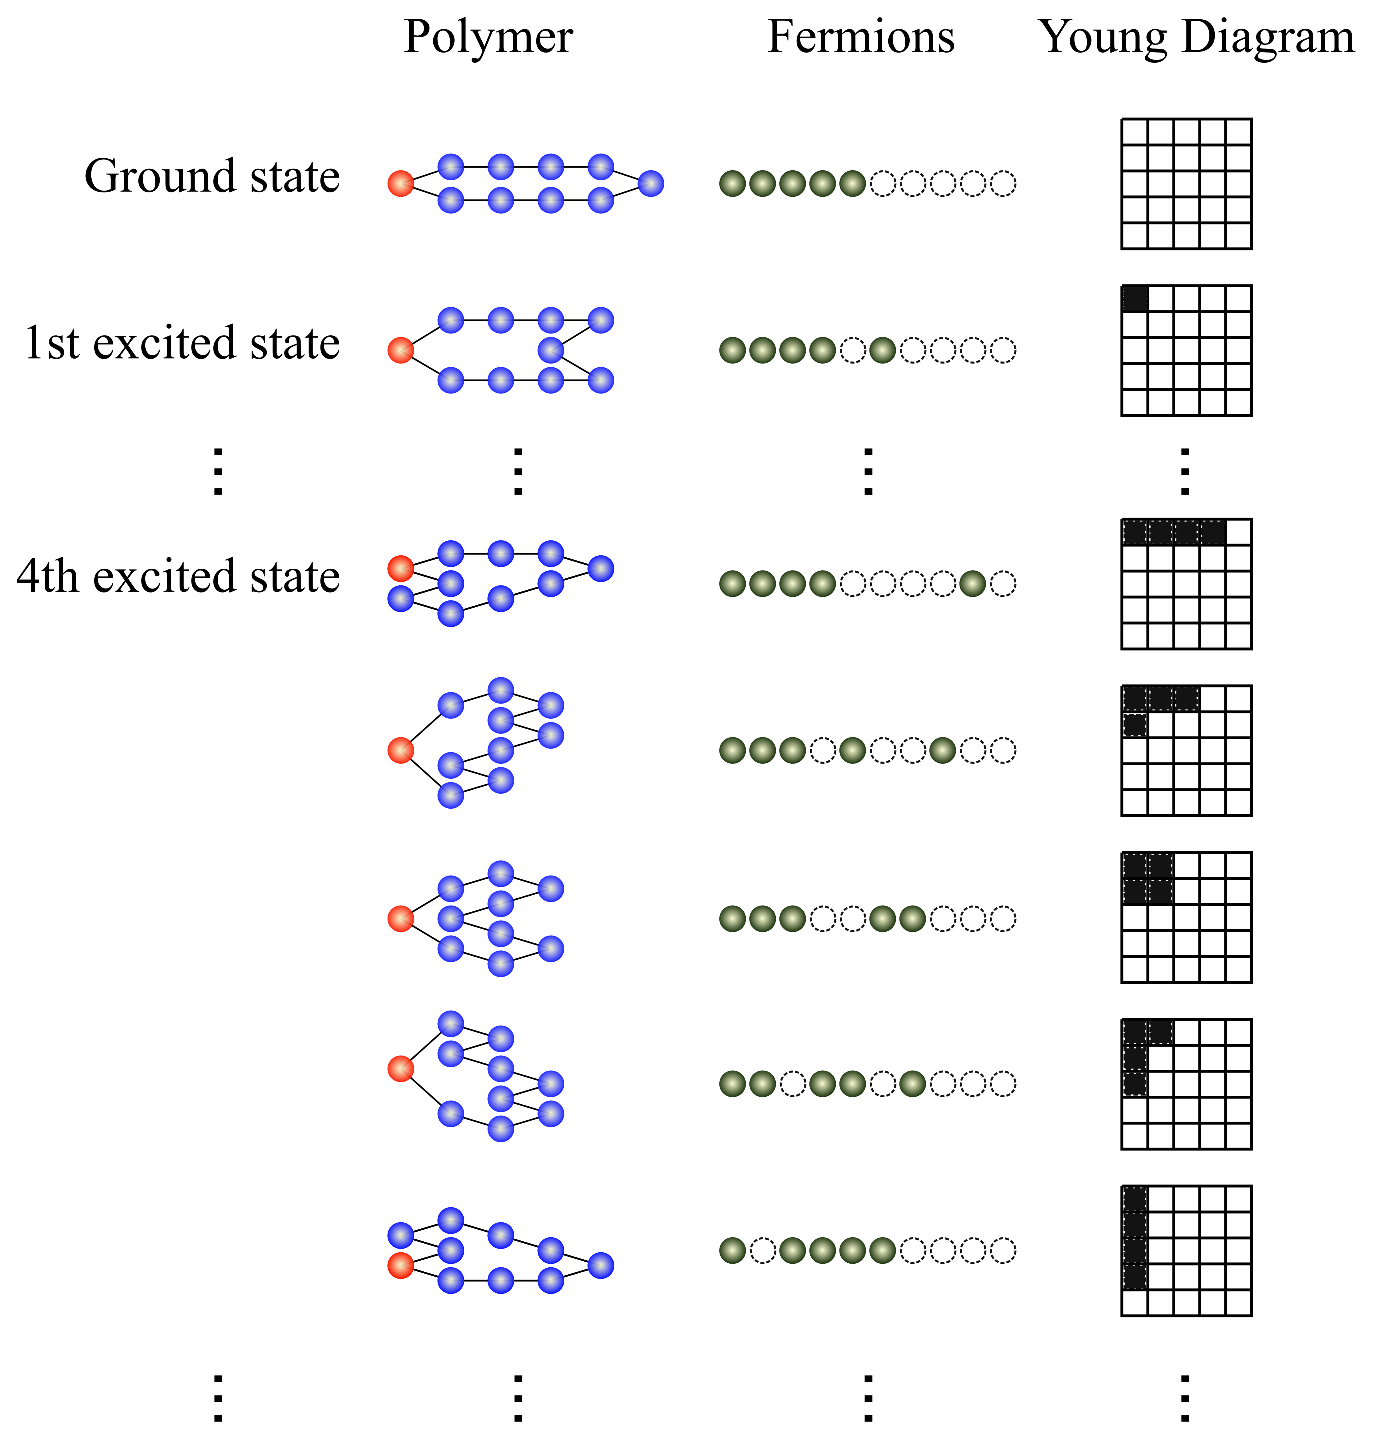
\includegraphics[width=0.45 \textwidth]{schematic.eps}
\caption{Schematic diagram. (a) Polymer blahblihblah (b) Fermion blahblihblah (c) Young diagram didadi...}
\label{fig:schematic}
\end{figure}

\section{Relation to integer partition and number theory} \label{sec:partition} 
Although the approach detailed in section \label{sec:FD} accurately estimates the mean and variance of equilibrium position of $j^{\rm}$ bead, it is an approximated theory. The random walk is continuous in space and the positions of the beads resides on an lattice. In addition, the distribution of the position of any bead in the random-walk picture is always a Gaussian \cite{klebaner2005introduction}, but in the discrete lattice model it is not: for example, in low temperature, the polymer would be mostly staying in its fully stretched configuration (see Fig.~\ref{fig:schematic}) and the distribution of the positions of the beads are always bounded by the natural length of the rods. 

Analytic solutions are possible in this particular model. We outline the key ideas in the followings, and leave the more detailed and technical analysis in a separate article [XXX]. 

Our idea is to change the basis of the Fermionic system from its microscopic configurations $\l\{Z_0,Z_1,\ldots,Z_{N-1}\r\}$ to the energy of the system. Clearly, the energy can only take values $E_0, E_0+\Delta E, \ldots, E_0 + N^2 \Delta E / 4$; in this picture, the probability space is a one-dimensional lattice with finite support. Without lost of generality, we let the constant energy $E_0=0$ and $\Delta E=1$ by choosing a proper unit. The difficulty of this basis is to determine the degeneracy of the microscopic states which have the same energy $E \in \l\{0,1,\ldots N^2/4\r\}$, sometimes referred to as the ``density of the state'' in statistical mechanics \cite{huang1987statistical} and condensed matter physics \cite{sander2009advanced}. We let the number of microscopic states with energy $E$ to be $g(E)$; once $g(E)$ is known, the partition function of the system can be formally derived in the canonical ensemble picture
\eq{
\mathcal{Z}\l(T\r) = \sum_{E=0}^{N^2/4} g(E) \, \exp \l(-\frac{E}{k_B T}\r),
}{eq:par_func}
and the equilibrium property of the system can be derived from $\mathcal{Z}$. 

With a little surprise, we discovered that $g(E)$ in this problem is closely related to the problem of integer partition in number theory \cite{andrews1998theory}. The connection can be made by formulating the problem in the following way. We consider to label the micro-state of the system by how many energy unit a Fermion is excited from its ground state. Mathematically, we denote $E_i$ to be the excited energy of the particle with $i^{\rm th}$ highest energy. The total energy of the system is
\begin{subequations} \label{eq:partition}
\begin{align}
E= \sum_{i=1}^{N} E_i,
\end{align}
and construction we have a constraint 
\begin{align}
N/2 \ge E_1 \ge E_2 \ge \ldots \ge E_{N/2} \ge 0. \label{eq:partition_constraint}
\end{align}
\end{subequations}
Equations \eqref{eq:partition} constitutes a restricted partition of the integer $E$: $g(E)$ is the possible ways to partition an integer $E$ into $N/2$ non-increasing parts \cite{andrews1998theory}.

A very neat way to label the microscopic configuration is to use the Young diagram \cite{andrews1998theory}, showing in the right panel of Fig.~\ref{fig:schematic}. The black box in row $i$ denotes the excited energy $E_i$. With the constraint \eqref{eq:partition_constraint}, each row can have at most $N/2$ black boxes, and the number of black boxes in $(i+1)^{\rm th}$ row cannot exceed the that in $i^{\rm th}$ row.  Then, $g(E)$ is the number of possibility of arrangement of $E$ black boxes onto the $N/2 \times N/2$ ``checkerboard''.

Once the this relation is identified, fruitful results from the number theory \cite{andrews1998theory} can be used to solve our problem. For example, denote  the ways to put $E$ black boxes onto an $K \times L$ checkerboard with non-increasing number of black boxes per row by $\pi \l(K,L,E\r)$. A recursive relation exists \cite{andrews1998theory}
\eq{
\pi\l(K,L,E\r) = \pi\l(K,L-1,E\r) + \pi \l(K-1,L, E-L\r),
}{}
which allows very efficient computations of the $g(E)=\pi\l(N/2,N/2,E\r)$. In addition, the generating function 
\eq{
\Phi \l(q\r) := \sum_{E=0}^{N^2/2} g(E) q^E
}{}
is identified to be the Gaussian binomial coefficient
\eq{
\Phi \l(q\r) \equiv \l(\begin{array}{c} N \\ N/2 \end{array}\r)_q := \frac{\prod_{j=1}^{N} \l(1-q^j\r)}{\l[\prod_{j=1}^{N/2} \l(1-q^j\r)\r]^2},
}{}
which allows us to formulate the partition function of the original polymer problem \eqref{eq:par_func}. 

We finally remark that along this line of analysis, the probability distribution analogous to \eqref{eq:discrete_prob} can also be formulated. Not surprisingly, for a finite (and small $N$), the exact results are different from \eqref{eq:discrete_prob}. Several other physical quantities at equilibrium can be efficiently computed without resorting to Monte Carlo simulation. We will present a more detailed analysis separately [XXX].  

\bibliography{refs}


\end{document}
